\section{Equational Reasoning}
\label{sec:equationalreasoning}

Verification is the process of checking if software does what it's specification demands. To verify a program, a specification is required. In the case of functions that implement an instance of the type classes of section \ref{sec:typeclasses}, the specification is defined in form of the type class laws.
This section will compare different verification techniques and describe the method equational reasoning by example using type class laws as specification. In section \ref{sec:example} equational reasoning will be applied to proof the property of listing \ref{lst:monoidinstance1} in section \ref{sec:typeclasses}.

There are several ways to check the behavior of a program. 
We will describe the difference with a simple example. Given the following property:

\begin{equation}
  \label{eq:reverse_prop}
\text{reverse} (\text{reverse } xs) = xs  
\end{equation}
Equation \ref{eq:reverse_prop} expresses, if we apply \verb|reverse| twice on the same list \verb|xs| we get back the original list \verb|xs|. \verb|reverse| is the inverse of \verb|reverse| (other functions, like \verb|id|, have this property too). Verification techniques allow us to check if equation \ref{eq:reverse_prop} holds. We describe three techniques. The first two, testing and property-based testing, are very common and the third is the topic of this article.

\begin{description}
\item[Testing] Run the program with a selected input and check if it behaves as expected. In order to check the behavior, a function evaluates both sides of the equation \ref{eq:reverse_prop} and compares the values. The following listing shows an example test.

\begin{lstlisting}[caption={Function definition for testing},label={lst:testing}]
input = [1,2,3]

test_reverse :: [Int] -> Bool
test_reverse xs = reverse (reverse xs) == xs
\end{lstlisting}

The selected input is \verb|[1,2,3]|. \verb|test_reverse| evaluates to a Boolean expression to indicate if the property holds for the given input. It's necessary to run the program to evaluate \verb|test_reverse|.
An advantage of this method is, that the programmer doesn't have to define general properties. The specification is expressed with a concrete input value and a concrete output value. It's easier to think about a concrete input and the corresponding output value than to find general properties that a function must obey.
\item[Property-based testing] The input for the test program is generated randomly. The tests are executed by a tool (e.g. Quickcheck).
\item[Proof] A Proof can show that a property holds in all circumstances. To prove a property we use the technique equational reasoning. This technique requires knowledge of the function definition.
\end{description}

Figure \ref{fig:property_validation} compares the input coverage of the described methods. Testing checks if the program behaves correctly with one chosen point of the input space. Property-based testing checks the behavior at hundreds of randomly-generated points. Proof covers all possible cases of the possible input. It is the most reliable verification.

\begin{figure}
  \centering
     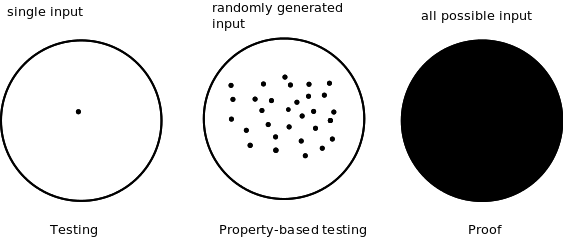
\includegraphics[width=0.9\textwidth]{testing}
  \caption{Comparison of testing, property-based-testing and proof}
  \label{fig:property_validation}
\end{figure}

\subsection{Reasoning about algebraic properties}

Equational reasoning is a method originally used in algebra. It's the process of proving a given property by substituting equal expressions.
For example, it's possible to show that the following property holds:
\begin{equation}
  \label{eq:sum}
  (x+a)(x+b) = x^2 + (a+b)x+ab
\end{equation}
To show that the equality holds, we have to transform the expression on the left-hand side  $(x+a)(x+b)$  to an equal expression on the right-hand side with the help of the basic algebraic properties of numbers (distributivity, commutative, associative, ) until we get $x^2 + (a+b)x+ab$  \cite{hutton}. 

In the first step (equation \ref{eq:firstalgebra} we use distributivity to expand the term on the left-hand side.
\begin{equation}
  \label{eq:firstalgebra}
  (x+a)(x+b) = x^2 + ax + xb + ab \text{     (use distributivity)}
\end{equation}
In the second step we use commutativity to substitute $xb$ with $bx$.
\begin{equation}
x^2 + ax + xb + ab = x^2 + ax + bx + ab \text{     (use commutativity)}
\end{equation}
In the last step we use distributivity to factorize $x$ and we get $x^2 + (a+b)x+ab$.
\begin{equation}
x^2 + ax + bx + ab = x^2 + (a + b)x + ab \text{     (use distributivity)}
\end{equation}
All we did, was substituting expression according the algebraic properties 

\subsection{Reasoning about Haskell programs}

A function definition in Haskell means that we can substitute the left-hand side with the right-hand side and vice versa. This is possible because Haskell is a purely functional language. Hence, we can use the same approach to prove that a property of a program written in Haskell holds, as we used to reason about mathematical expressions. 
For example, it's possible to show that the length of a list with one element is actually 1. This general property can be formed as boolean expression in Haskell.
\begin{verbatim}
length [x] == 1
\end{verbatim}
The property holds no matter what \verb|x| is. To show that, we use the \gls{function-definition} of \verb|length| as a general description of the behavior. Listing \ref{lst:lengthdefinition} shows the definition of \verb|length| \cite{hutton}.
\begin{lstlisting}[caption={Function definition of length},label={lst:lengthdefinition}]
length [] = 0
length (x:xs) = 1 + length xs  
\end{lstlisting}

To conclude that \verb|length [x] == 1| is always true, we substitute \verb|length [x]| until we get \verb|1|. Listing \ref{lst:lengthproof} shows the step by step substitution.
\begin{lstlisting}[caption={Deduce that the length of a list with one element is 1},label={lst:lengthproof}]
length [x] = 
length (x:[])   -- [x] is the same as x:[]
1 + length []   -- apply definition
1 + 0           -- apply defintion
1               -- 1 + 0 = 0
\end{lstlisting}
Function definitions are general description and we can use them to deduce other general properties by substituting equal expressions.

\subsection{Proof by structural induction}
\label{sec:induction}

If we apply simple substitution to a recursive function, we run into problems.
Consider the \gls{function-definition} of \verb|length| in listing \ref{lst:lengthdefinition}.
If we substitute \verb|length x| with the definition \verb|1 + length xs|, we end up substituting \verb|length x| forever. A way to verify recursive programs is to use proof by structural induction.  
Structural induction for proofing a property can be used for list or algebraic data types with a recursive constructor (e.g. Tree).

 The principle of induction states, that it is sufficient to prove a property $p$ for the base case and that $p$ is preserved by the inductive case. In order to prove $p$, two steps are required:
 \begin{description}
 \item[Base case] Prove $p(0)$ is true.
 \item[Induction step] Prove $p(n+1)$ if $p(n)$ (induction hypothesis) is true.
 \end{description}

Proof by induction is similar to writing a recursive function. Recursive functions use a base case (e.g. \verb|[]|, 0). 
If we use structural induction we proof the base case. We show that the property holds for a concrete input value (e.g. \verb|[]|, 0). 

In a recursive function definition we define \verb|f (x:xs)| and use \verb|f x| in the right-hand side. In the proof we show that $p(n+1)$ with the assumption $p(n)$.

We explain proof by structural induction with another example. We verify that the overall length of two concatenated lists $xs$ and $ys$, is the same as the sum of the length of $xs$ and the length of $ys$.  The ++-operator concatenates two lists.
\begin{equation}
  \label{eq:lengthprop}
  \text{length (xs ++ ys)} = \text{(length xs) + (length ys)}
\end{equation}
In order to verify property \ref{eq:lengthprop}, we need the function definitions for \verb|length| and \verb|(++)|.
The Prelude functions \verb|length| and \verb|(++)| are given in listing \ref{lst:lengthdefinition} and \ref{lst:concatdefintion}.

\begin{lstlisting}[caption={Haskell function definition of the concatenation operator},label={lst:concatdefintion}]
[] ++ xs = xs
(x:xs) ++ ys = x:(xs++ys)
\end{lstlisting}

\begin{description}
\item[Base case]
We have to show that property \ref{eq:lengthprop} holds for the base case. The base case, in this example, are the arguments \verb|[]| and an arbitrary list for \verb|ys|. It isn't necessary to replace \verb|ys| because the definition of \verb|++| uses recursion over \verb|xs|. \verb|ys| will always be the same list.
In order to check if property \ref{eq:lengthprop} holds for the base case, we replace \verb|xs| with  \verb|[]|, leading to

\begin{verbatim}
length ([] ++ ys) == length [] + length ys
\end{verbatim}

We will evaluate the expression on the left-hand side and the right and side separately.
The left-hand side evaluates to

\begin{verbatim}
length ([] ++ ys) -- apply ++
length ys
\end{verbatim}

The right-hand side evaluates to 

\begin{verbatim}
length [] + length ys     -- apply length []
0 + length ys
length ys
\end{verbatim}

When we evaluate each side of the equation \ref{eq:lengthprop} with the value \verb|[]| for \verb|xs|, the result is \verb|length ys| on both sides. Hence, property \ref{eq:lengthprop} holds for the base case.

\item[Induction step]
 We have to prove that the two expressions on both sides of the \verb|=| sign in listing \ref{lst:inductionstep} are equal
\begin{lstlisting}[caption={The left-hand side and the right-hand side have to be equal},label={lst:inductionstep}]
length ((x:xs) ++ ys) = length (x:xs) + (length ys)
\end{lstlisting}

with the assumption (induction hypothesis).
\begin{equation}
  \label{eq:induction_hypothesis}
      \text{length(xs ++ ys)} = \text{length(xs) + length(ys)}
\end{equation}

Again, we evaluate the the left-hand side of equation in listing \ref{lst:inductionstep}.

\begin{program}
\begin{verbatim}
length ((x:xs) ++ ys)     --apply definition of ++
length (x:(xs ++ ys))      --apply definition of length
1 + length (xs ++ ys)      --use induction hypothesis
1 + length xs + length ys
\end{verbatim}
\end{program}

If we evaluate the right-hand side of the equation in listing \ref{lst:inductionstep} we get:
\begin{program}
\begin{verbatim}
length (x:xs) + length ys    -- apply definition of length
1 + length xs + length ys
\end{verbatim}
\end{program}

The last listing shows, that the equality in listing \ref{lst:inductionstep} follows from the induction hypothesis in equation \ref{eq:induction_hypothesis}. This completes the induction step and therefore the proof itself.
\end{description}

The previous example used \glspl{function-definition} of \verb|length| and \verb|(++)|. In order to apply equational reasoning we have to know the function definitions of involved functions or we can rely on already proven properties. 
For example all types of the standard library, that are an instance of a type class, satisfy the type class laws (see \ref{sec:typeclasses}) \cite{yorgey}. Some libraries exhibit properties in their documentation (e.g. pipes library \cite{gonzales13}). 